%%
\chapter{Generating query based monitoring components}
%%

After the domain model of the system is designed, and the graph queries are written, the monitoring components can be generated and deployed along with \cpp{} tools for modeling the domain.
As stated before, domain modeling and graph query definition are done using EMF and \viatra{} technologies.
In this chapter, I present how the monitoring components are generated from these artifacts.

From the metamodel, the framework generates the classes, which enables the programmer to model the system's state in \cpp{}.
Also, we generate the monitoring code for the system, which is basically the \cpp{} version of the planned graph queries. 
These graph queries are evaluated on the maintained \cpp{} model.

\section{Generating classes from the metamodel}

The domain model consists of packages (EPackage), enumerations (EEnum) and classes (EClass).
From an EPackage, we generate a folder and every source file originated from the elements of the package will be generated in that folder. 
We generate sources from each class and enumeration of the package, also we generate other artifacts for the package.


\subsection{Mapping an EClass to \protect\cpp }


\todo{ábra szépítés}
\begin{figure}
	\begin{center}
		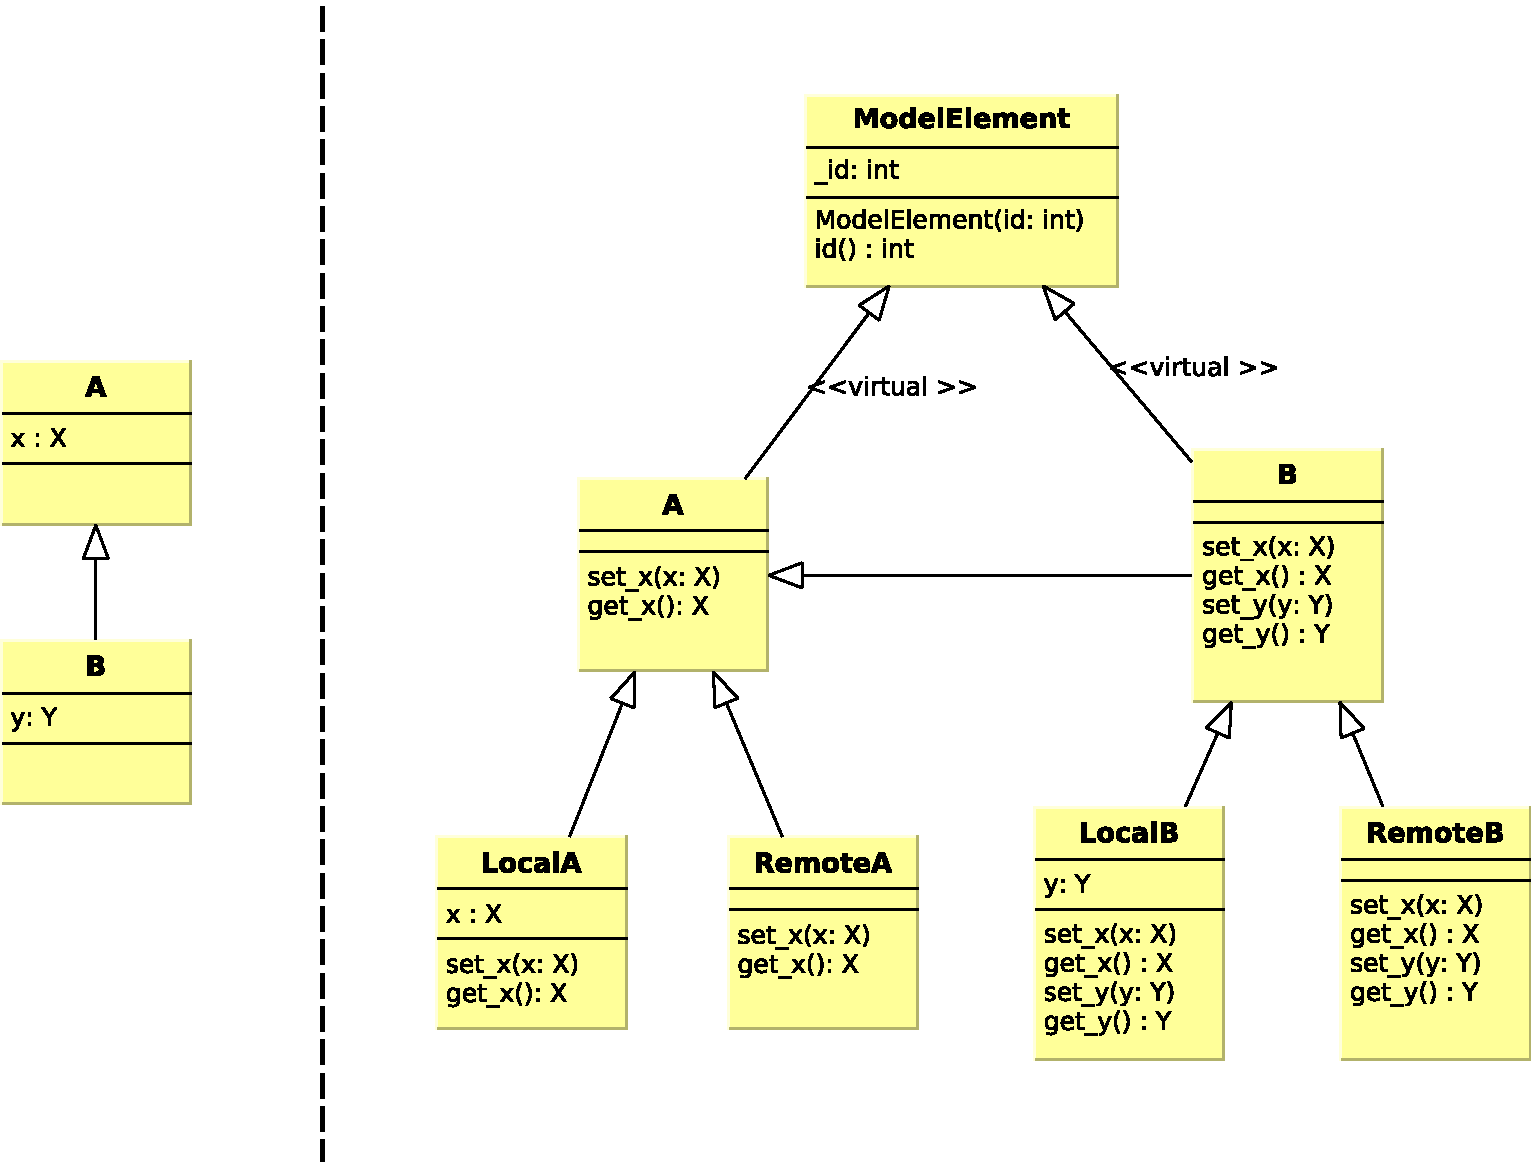
\includegraphics[width=\textwidth]{figures/eclass-to-cpp.pdf}
		\caption{Mapping of two EClasses, one inherited from the other (Left: EClasses, right: \protect\cpp{} classes) }
		\label{fig:eclass-to-cpp}
	\end{center}
\end{figure}


The EClasses of the metamodel are mapped to various \cpp{} classes, as depicted on \mbox{Figure~\ref{fig:eclass-to-cpp}}.
From each EClass we generate three \cpp{} classes:

\begin{itemize}
	\item An interface (abstract class with only pure virtual methods in \cpp{})
	\item A local class
	\item A remote class
\end{itemize}


The interface provides access to an instance of the EClass.
The local class implements the interface. It stores the attributes and references of the instances allocated to the local computing unit, and made them accessible by the methods of the implemented interface.
The remote class implements the interface, but are only used to substitute remote objects in references to them; 
Accessing its variables are not possible, because they are stored in another node. 

\subsection{Mapping an EEnum to \protect\cpp }

Enumerations are simply mapped to \cpp{} enum classes as depicted on Fig.\ref{fig:eenum-to-cpp}.

\begin{figure}[H]
	\begin{center}
		
		\begin{minipage}[c]{\textwidth}
		\begin{minipage}[r]{0.52\textwidth}
			\hfill
			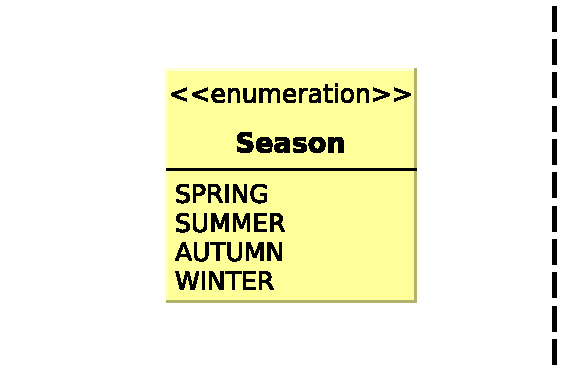
\includegraphics[width=0.735\textwidth]{figures/eenum-to-cpp.pdf}
		\end{minipage}
			\hspace{0.05\textwidth}
		\begin{minipage}[c]{0.25\textwidth}
\begin{lstlisting}[language=C++]
namespace Package{

enum class Season{
	SPRING = 0,
	SUMMER = 1,
	AUTUMN = 2,
	WINTER = 3
};

}
\end{lstlisting}			
		\end{minipage}
		\end{minipage}
		\caption{Mapping of an enumeration to \protect\cpp{} enum class }
		\label{fig:eenum-to-cpp}
	\end{center}
\end{figure}

\subsection{ Generating ModelRoot class and utilities }


\todo{MEGÍRNI}





\section{Overview of the query compilation workflow}

The compilation of the queries of the CPS is depicted in fig. \ref{figure:query-compile-workflow}. 
First, vql files are parsed using EMF so its content is loaded into a Pattern Model.
The Pattern Model are processed by \viatra{} and converted into PSystem representation of queries.
After that, we extend this representation with type information, as type information is important in the \cpp{} generated code.
Then, we create the plan for query execution; We use the local search planner of \viatra{} fine tuned with our search operation cost function to improve performance of distributed queries. 
We also use some optimizations later to improve distributed performance. 
After the fully optimized plan is ready, we can construct the generator model describing the source code structure and generate the \cpp{} files.


\begin{figure}[h]
	\begin{center}
		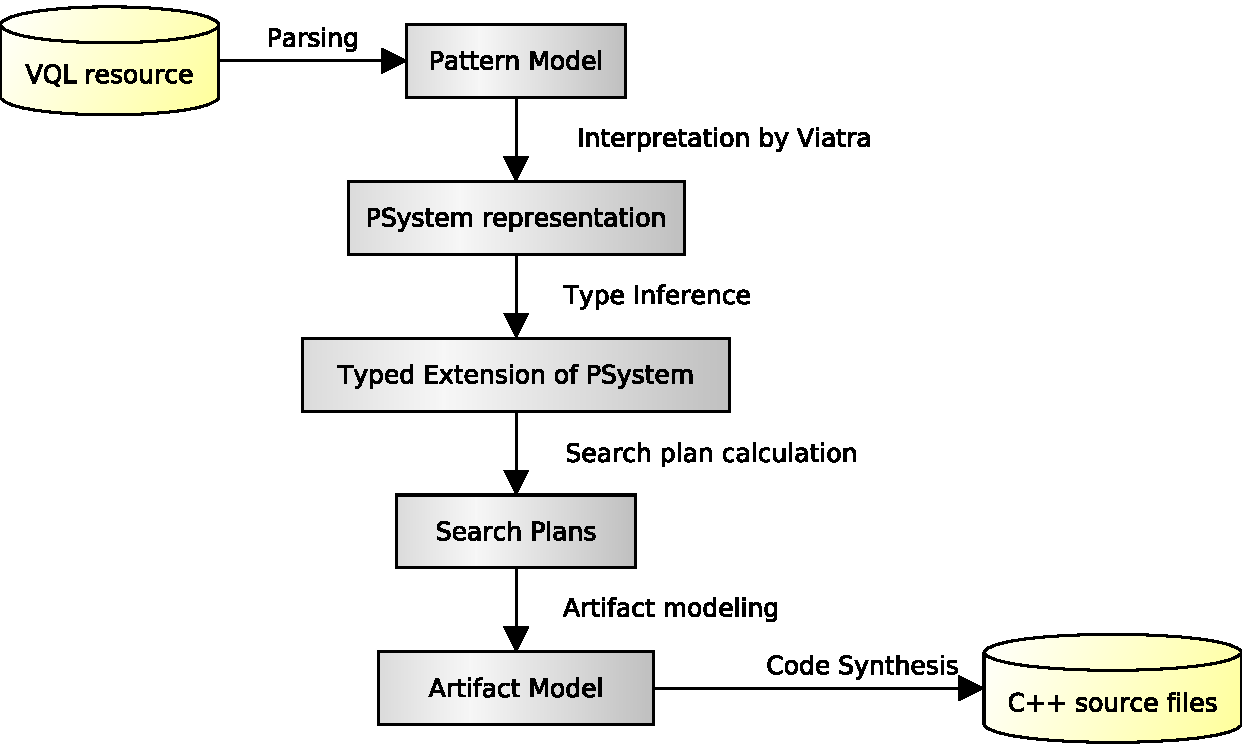
\includegraphics[width=0.8\textwidth]{figures/query-compilation-workflow.pdf}
		\caption{Query compilation workflow}
		\label{figure:query-compile-workflow}
	\end{center}
\end{figure}



\section{Viatra plan}

The query file is processed by \viatra{}~\cite{viatra} and a local search plan is generated. 
The local search planner of \viatra{} can be customized by specifying a cost function
In case of local search, the plan is a sequence of search operation defined as an application of a constraint.

\section{Completed plan}

\viatra{} generated plans are not intended for external usage. 
We need to complete it with additional information to use it for our purposes. 
One of the main concern is type information. To obtain type information we use the constraints to deduce the type of a variable. 


\section{Additional optimization}

After we complete the plan with type information and other details, it can be used to generate C++ code, although before that step we use further optimizations. 
These optimizations considers distributed execution of the plan, so it can improve the plan generated by \viatra{} which is generated to be used in a single computer.


\subsection{Replace pattern calls with simpler operations}
There are some cases, where helper patterns are simple, and used to define simple conditions. 
In this case, evaluationg the subquery is not always the most efficient method, sometimes these can be replaced by simple search operations:

\subsubsection{Reference Pattern}
We use the phrase \emph{reference pattern} for a pattern with 2 parameters if its only constraint is that a reference exist between the two parameters, eg.:
\begin{lstlisting}[language = vql]
private pattern connected(a : RailRoadElement, b : RailRoadElement){
	RailRoadElement.connectedTo(a,b);
}
\end{lstlisting}

In the following examples i will use this query as an example to demonstrate how the application of this query can be replaced by an other operation.

\subsubsection{Counting reference pattern}
\begin{lstlisting}[language = vql]
1 == count find connected(a, _);
\end{lstlisting}


\subsubsection{Negative application of a reference pattern}

\begin{lstlisting}[language = vql]
neg find connected(a, _);
\end{lstlisting}

\subsection{Filter unnecessary operations, checks}
As the original plan is generated by the localsearch planner of \viatra{}, there can be redundant operations, which can be ommited. This includes:

\begin{itemize}
	\item Check operation -- The generated code is strongly typed, so we don't need type checks in most cases, unlike in the Java implementation, where the tuples contains plain java objects with unknown types.
	
	\item Distribution operations -- \todo{KIFEJTENI}
\end{itemize}



\section{C++ code generation}

The completed and optimized plan are used to generate \cpp{} code. 
Two main methods can be used to run local search plan in case of generated code. 
One is to generate the plan as a data structure and create an interpreter that uses that plan to find matches. 
The other is to generate the code directly from the plan. 
The first method is good if we want to change the plan at runtime, but the interpreter itself introduces an overhead, causing performance to be slower.
We used the later, because we don't change the plan at runtime.












